%%%%%%%%%%%%%%%%%%%%%%%%%%%%%%%%%%%%%%%%%
% Beamer Presentation
% LaTeX Template
% Version 1.0 (10/11/12)
%
% This template has been downloaded from:
% http://www.LaTeXTemplates.com
%
% License:
% CC BY-NC-SA 3.0 (http://creativecommons.org/licenses/by-nc-sa/3.0/)
%
%%%%%%%%%%%%%%%%%%%%%%%%%%%%%%%%%%%%%%%%%

%----------------------------------------------------------------------------------------
% PACKAGES AND THEMES
%----------------------------------------------------------------------------------------

\documentclass{beamer}
% \usepackage{courier}
\usepackage{hyperref}
\usepackage{url}
\usepackage{ulem}
\usepackage{tikz}
\usepackage{multicol}
\usetikzlibrary{fit,calc,positioning,decorations.pathreplacing,matrix}
\usetikzlibrary{positioning}
\usepackage{algorithm}% http://ctan.org/pkg/algorithms
\usepackage{algorithmic}
\usepackage{cleveref}
\usepackage{caption}
\usepackage{appendixnumberbeamer}
\usepackage[latin1]{inputenc}
\usetikzlibrary{shapes, arrows, calc, positioning}

\tikzstyle{block} = [rectangle, draw, fill=blue!20,
    text width=10em, text centered, rounded corners, minimum height=1em, node distance=1em]
\tikzstyle{method} = [text width=8em, midway, right]
\tikzstyle{line} = [draw, -latex']
\tikzstyle{edge} = [draw, -, color=red]
\tikzstyle{cloud} = [draw, ellipse, fill=red!20, node distance=1em,
    minimum height=1em]
\tikzstyle{input} = [rectangle, draw,
    text width=3em, text centered, rounded corners, minimum height=1em, node distance=1em]
\tikzstyle{output} = [rectangle, draw,
    text width=3em, text centered, rounded corners, minimum height=1em, node distance=1em]
\tikzstyle{dnn} = [rectangle, draw,  fill=gray!20,
    text width=12em, text centered, rounded corners, minimum height=8em, node distance=1em]

\addtobeamertemplate{navigation symbols}{}{%
    \usebeamerfont{footline}%
    \usebeamercolor[fg]{footline}%
    \hspace{1em}%
    \insertframenumber/\inserttotalframenumber
}

\mode<presentation> {

% The Beamer class comes with a number of default slide themes
% which change the colors and layouts of slides. Below this is a list
% of all the themes, uncomment each in turn to see what they look like.

\usetheme{default}
%\usetheme{AnnArbor}
%\usetheme{Antibes}
%\usetheme{Bergen}
%\usetheme{Berkeley}
%\usetheme{Berlin}
%\usetheme{Boadilla}
%\usetheme{CambridgeUS}
%\usetheme{Copenhagen}
%\usetheme{Darmstadt}
%\usetheme{Dresden}
%\usetheme{Frankfurt}
%\usetheme{Goettingen}
%\usetheme{Hannover}
%\usetheme{Ilmenau}
%\usetheme{JuanLesPins}
%\usetheme{Luebeck}
%\usetheme{Madrid}
%\usetheme{Malmoe}
%\usetheme{Marburg}
%\usetheme{Montpellier}
%\usetheme{PaloAlto}
%\usetheme{Pittsburgh}
% \usetheme{Rochester}
%\usetheme{Singapore}
%\usetheme{Szeged}
%\usetheme{Warsaw}

% As well as themes, the Beamer class has a number of color themes
% for any slide theme. Uncomment each of these in turn to see how it
% changes the colors of your current slide theme.

%\usecolortheme{albatross}
%\usecolortheme{beaver}
%\usecolortheme{beetle}
%\usecolortheme{crane}
%\usecolortheme{dolphin}
%\usecolortheme{dove}
%\usecolortheme{fly}
%\usecolortheme{lily}
%\usecolortheme{orchid}
%\usecolortheme{rose}
%\usecolortheme{seagull}
%\usecolortheme{seahorse}
%\usecolortheme{whale}
%\usecolortheme{wolverine}

%\setbeamertemplate{footline} % To remove the footer line in all slides uncomment this line
%\setbeamertemplate{footline}[page number] % To replace the footer line in all slides with a simple slide count uncomment this line

%\setbeamertemplate{navigation symbols}{} % To remove the navigation symbols from the bottom of all slides uncomment this line
}

\usepackage{graphicx} % Allows including images
\usepackage{booktabs} % Allows the use of \toprule, \midrule and \bottomrule in tables

\newcommand\logit{\text{logit}}
\usepackage{amsmath}
%----------------------------------------------------------------------------------------
% TITLE PAGE
%----------------------------------------------------------------------------------------

\title{Testing epistatic effect in complex trait using related intermediate trait} % The short title appears at the bottom of every slide, the full title is only on the title page
\author{Yanyu Liang}
\institute[U of C]
{
University of Chicago \\
\medskip
\textit{yanyul@uchicago.edu} % Your email address
}
\date{\today} % Date, can be changed to a custom date

\begin{document}

\begin{frame}
\titlepage % Print the title page as the first slide
\end{frame}
\addtocontents{toc}{\setcounter{tocdepth}{1}}
\begin{frame}
% \begin{multicols}{2}
\frametitle{Overview} % Table of contents slide, comment this block out to remove it
\tableofcontents % Throughout your presentation, if you choose to use \section{} and \subsection{} commands, these will automatically be printed on this slide as an overview of your presentation
% \end{multicols}
\end{frame}

%----------------------------------------------------------------------------------------
% PRESENTATION SLIDES
%----------------------------------------------------------------------------------------

%------------------------------------------------
\section{Background}
%------------------------------------------------

  \subsection{Mendelian disease and complex trait}
  \begin{frame}
  \frametitle{Mendelian disease and complex trait}
    \begin{columns}
      \begin{column}{.49\textwidth}
        \begin{itemize}
          \item Caused by single variant on a gene (or regulatory region), \textit{i.e.} Phenylketonuria is caused by abnormal \textit{PAH} gene which encodes phenylalanine hydroxylase
          \item Highly heritable and is inherited in recessive or dominant way, \textit{i.e.} Mendel's laws
          \item They are in general rare
        \end{itemize}
      \end{column}
      \begin{column}{.49\textwidth}
        \begin{itemize}
          \item Caused by many variants along with environmental factors, \textit{i.e.} high blood pressure, type II diabetes
          \item Also heritable but no clear pattern of recessive or dominant
          \item They are more common in population, \textit{i.e.} more than 30\% people (older than 20) have high blood pressure in U.S.
        \end{itemize}
      \end{column}
    \end{columns}
  \end{frame}

  \subsection{GWAS and complex trait}
  \begin{frame}
  \frametitle{GWAS and complex trait}
    \centering
    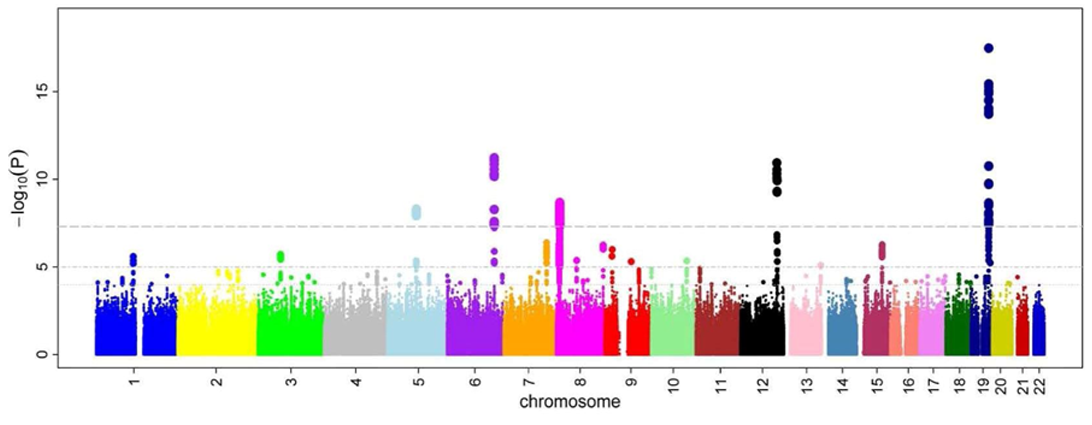
\includegraphics[width=0.8\linewidth]{gwas}
    \label{fig:gwas}
    \begin{itemize}
      \item Genome-wide association study (GWAS)
      \begin{itemize}
        \item Case-control study
        \item Look for association between disease status and genotype
        \item Perform test each locus at a time
      \end{itemize}
      \item GWAS has been extensively used to identify causal genes for complex trait
  \end{itemize}
  \end{frame}

  \subsection{Genetic background and disease}
  \begin{frame}
  \frametitle{Genetic background and disease}
    \begin{itemize}
      \item Carrying pathogenic variant may not lead to disease, \textit{incomplete penetrance} (ExAC \cite{lek2016analysis})
      \item In complex trait, risk loci only explain a small fraction of disease risk
      \item Explanations
        \begin{itemize}
          \item Rare variant also contribute
          \item Weak effect loci also contribute additively (polygenic assumption)
          \item The effect of risk loci depends on other loci non-additively (epistatic effect of genetic background)
        \end{itemize}
    \end{itemize}
  \end{frame}

  \subsection{Epistatic effect - an example of color coating}
  \begin{frame}
  \frametitle{Epistatic effect - an example of color coating \cite{phillips2008epistasis}}
    \begin{columns}
      \begin{column}{.44\textwidth}
        \centering
        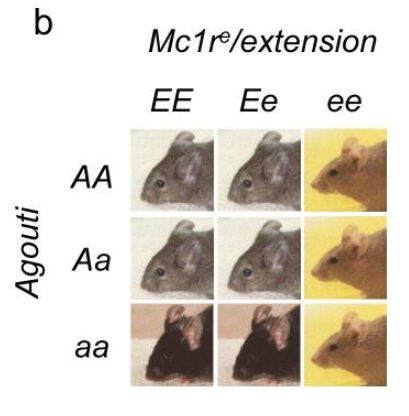
\includegraphics[width=\linewidth]{epi}
        \label{fig:epi}
        \begin{itemize}
          \item The effect of $Agouti$ is masked by $Mc1r^e$
        \end{itemize}
      \end{column}
      \begin{column}{.54\textwidth}
        \centering
        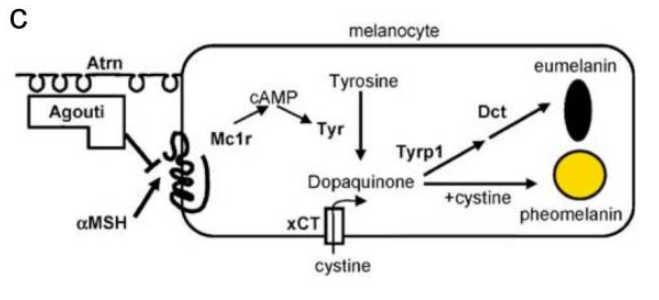
\includegraphics[width=\linewidth]{epi2}
        \label{fig:epi2}
        \begin{itemize}
          \item In the pathway $Agouti$ is upstream of $Mc1r^e$ and the phenotypic effect of $Agouti$ acts through $Mc1r^e$. So, when $Mc1r^e$ loses function, $Agouti$ 'loses' its effect
        \end{itemize}
      \end{column}
    \end{columns}
  \end{frame}

  \subsection{Epistatic effect}
  \begin{frame}
  \frametitle{Epistatic effect}
    \begin{itemize}
      \item Epistasis occurs when the effect of one gene depends on other genes, modifiers ($Agouti$ depends on $Mc1r^e$ to have normal function)
      \item More generally, the effect of loci as a whole is different from their individual effect
    \end{itemize}
  \end{frame}

  %------------------------------------------------
  \section{Motivation}
  %------------------------------------------------

    \subsection{Question}
    \begin{frame}
    \frametitle{Question}
      \begin{enumerate}
        \item In complex trait, is there any epistatic effect?
        \item If so, how to identify them from current data?
      \end{enumerate}
    \end{frame}

    \subsection{Ideas}
    \begin{frame}
    \frametitle{Ideas}
      \begin{enumerate}
        \item Beside the epistatic signals that have already be found by performing SNP-SNP interaction test, epistatic effect makes biological sense.
          \begin{itemize}
            \item Molecules in the same pathway may act depending on each others
            \item The outcome of one pathway may modify the effect of the gene in another pathway
          \end{itemize}
        \item Currently, SNP-SNP interaction is computationally tractable but with huge statistically burden. It is better to shrink SNP searching space and aggregate signals in some way (hypothesis-based)
      \end{enumerate}
    \end{frame}

    \subsection{Hypothesis}
    \begin{frame}
    \frametitle{Hypothesis}
      For some complex trait, the related pathway (let say they are \textbf{intermediate traits}) is known. And these intermediate traits potentially modify the effect of risk gene. For instances,
        \begin{itemize}
          \item Low density lipo-protein (LDL) level may modify coronary heart disease (CHD) risk
          \item The sensitivity of immune system (baseline activity) may modify Crohn's disease (CD) risk
          \item Baseline glucose level may modify type II diabetes (T2D) risk
        \end{itemize}
    \end{frame}

%------------------------------------------------
\section{Method}
%------------------------------------------------

  \subsection{Method overview}
  \begin{frame}
  \frametitle{Method overview}
    \begin{columns}
      \begin{column}{.44\textwidth}
        \begin{itemize}
          \item Polygenic risk score (PRS) is computed from genotype data
          \item Obtain a set of loci which are potentially modified by the intermediate trait
          \item Test interaction between $\hat{I}$ and $X_j$ on the disease risk $Y$
        \end{itemize}
      \end{column}
      \begin{column}{.54\textwidth}
        \begin{itemize}
          \item LDpred \cite{vilhjalmsson2015modeling} is used to obtain posterior mean effect $\bar{\beta}_i$ and $\hat{I} = \sum_i \bar{\beta}_i X_i$
          \item i) GWAS significant SNPs; \\
                ii) SNPs that are likely to act through the intermediate trait
          \item $\logit{\Pr(Y = 1|\hat{I}, X_j)} = \alpha + \beta_I \hat{I} + \beta_j X_j + \gamma \hat{I} X_j$ using \texttt{plink}
        \end{itemize}
      \end{column}
    \end{columns}
  \end{frame}

  \subsection{Data overview}
  \begin{frame}
  \frametitle{Data overview}
    \begin{itemize}
      \item Genotype of a case-control study, WTCCC (2009) \cite{wellcome2007genome}
        \begin{itemize}
          \item Three diseases along with two shared controls: CHD, CD, T2D (sample size 4000-5000 each)
        \end{itemize}
      \item Summary statistic of intermediate traits
        \begin{enumerate}
          \item LDL, HDL, triglycerides (TG) \cite{kettunen2016genome}
          \item Insulin-like growth factor 1 (IGF1) \cite{prins2017genome}
          \item White blood cell count (WBC) \cite{astle2016allelic}
          \item Fast glucose, fast insulin \cite{manning2012genome}
        \end{enumerate}
    \end{itemize}
  \end{frame}

%------------------------------------------------
\section{Results}
%------------------------------------------------

  \subsection{Intermediate trait PRS is correlated with disease status}
  \begin{frame}
  \frametitle{Intermediate trait PRS is correlated with disease status}
    We first test whether intermediate trait PRS $\hat{I}$ is correlated with the disease of interest $Y$. The following pairs are tested
    \begin{itemize}
      \item CHD vs. LDL, HDL, TG
      \item CD vs. IGF1, WBC
      \item T2D vs. FastGlu, FastInsulin
    \end{itemize}
    In short, we find the following significant association (p-value $<$ 0.05) under $\logit(\Pr(Y = 1|\hat{I})) = \alpha + \beta \hat{I}$
    \begin{itemize}
      \item CHD $\leftarrow^{-}$ LDL, CHD $\leftarrow^{+}$ TG, HDL (n.s.)
      \item CD $\leftarrow^{+}$ WBC, IGF1 (n.s.)
      \item T2D $\leftarrow^{+}$ FastGlu, T2D $\leftarrow^{+}$ FastInsulin
    \end{itemize}
  \end{frame}

  \subsection{Test interaction on GWAS significant hits: CHD - LDL}
  \begin{frame}
  \frametitle{Test interaction on GWAS significant hits: CHD - LDL}
    \centering
    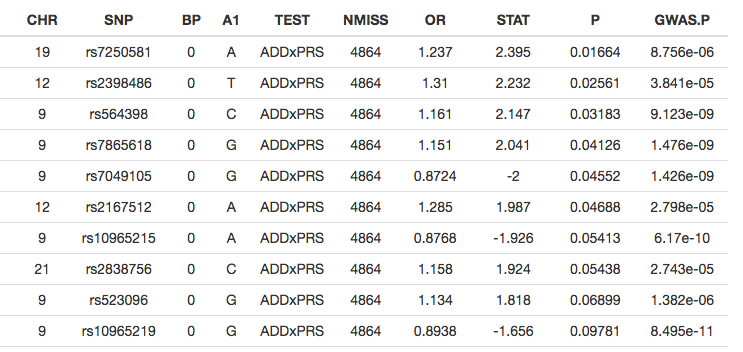
\includegraphics[width=.8\linewidth]{ldl}
    \label{fig:ldl}
    \begin{itemize}
      \item Most of them locate near CDKN2B antisense RNA 1 (\textit{CDKN2B-AS1}) and the rest is at \textit{TMEM132D} region, with little effect on LDL
      \item The effect of the locus is masked by high LDL level (namely the sign of $\beta_j$ is opposite to $\gamma$)
    \end{itemize}
  \end{frame}

  \subsection{Test interaction on GWAS significant hits: CD - WBC}
  \begin{frame}
  \frametitle{Test interaction on GWAS significant hits: CD - WBC}
    \centering
    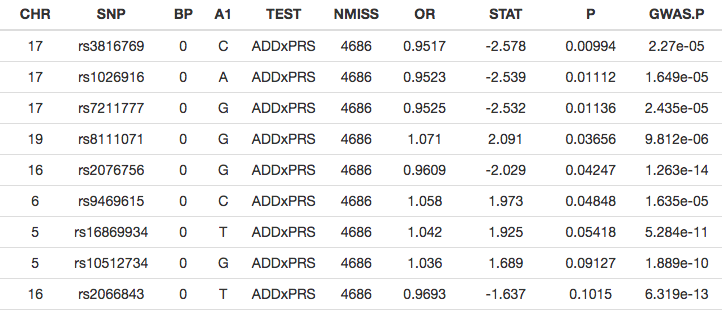
\includegraphics[width=.8\linewidth]{wbc}
    \label{fig:wbc}
    \begin{itemize}
      \item Some loci locate near \textit{NOD2} (IBD gene), \textit{STAT3} (related o immune response), with little effect on WBC
      \item The effect of the \textit{NOD2} locus is masked by high WBC level
      \item The effect of the \textit{STAT3} locus is enhanced by high WBC level (namely the sign of $\beta_j$ is the same as $\gamma$)
    \end{itemize}
  \end{frame}

  \subsection{Test interaction on GWAS significant hits: T2D - FastInsulin}
  \begin{frame}
  \frametitle{Test interaction on GWAS significant hits: T2D - FastInsulin}
    \centering
    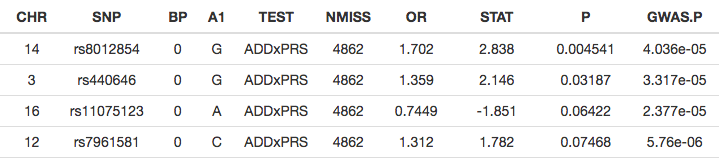
\includegraphics[width=.8\linewidth]{insulin}
    \label{fig:insulin}
    \begin{itemize}
      \item \textit{rs440646} locates in the intronic region of \textit{HRH1} which acts as a stimulator of insulin-induced adipogenesis
      \item It has little effect to fast insulin level and the effect on T2D is enhanced by high fast insulin level
    \end{itemize}
  \end{frame}

  \subsection{Test interaction on SNPs that potentially act through the intermediate trait}
  \begin{frame}
  \frametitle{Test interaction on SNPs that potentially act through the intermediate trait}
    \centering
    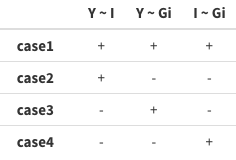
\includegraphics[width=.45\linewidth]{consistent}
    \label{fig:consistent}
    \hfill
    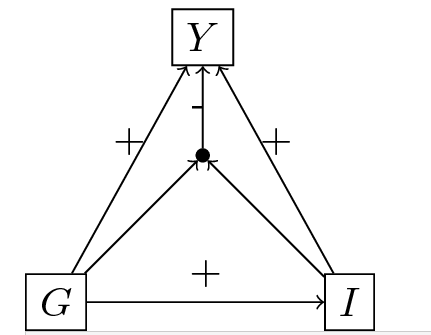
\includegraphics[width=.45\linewidth]{example}
    \label{fig:example}
    \begin{itemize}
      \item If SNP acts through the pathway, it is likely to be modified by the pathway
      \item The marginal effect of SNP on disease and SNP on intermediate trait should be consistent with the effect of intermediate trait on disease
      \item We collect SNPs that act consistently as a \textbf{consistent} set
    \end{itemize}
  \end{frame}

  \subsection{Test interaction on consistent SNPs: CHD - LDL}
  \begin{frame}
  \frametitle{Test interaction on consistent SNPs: CHD - LDL}
    \centering
    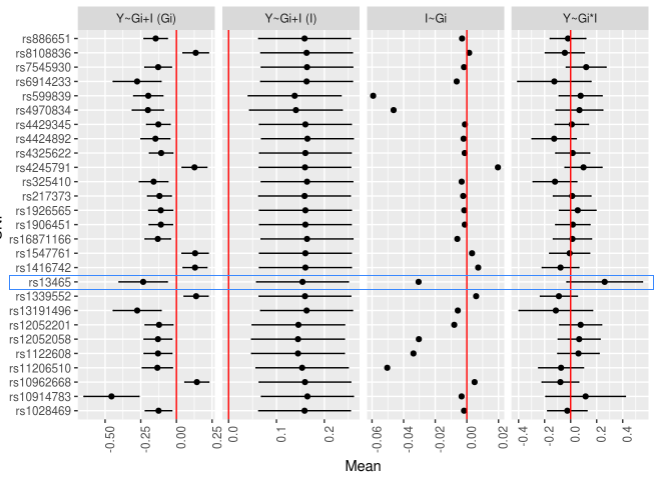
\includegraphics[width=.8\linewidth]{ldl2}
    \label{fig:ldl2}
    \begin{itemize}
      \item \textit{rs13465} locates in the intronic region of \textit{ILF3}. Its protective effect is masked by high LDL level
      \item Interestingly, it has been reported that \textit{ILF3} affects myocardial infarction risk only when LDL level is low \cite{yoshida2011association}.
    \end{itemize}
  \end{frame}

  \subsection{Test interaction on consistent SNPs: T2D - FastGlu}
  \begin{frame}
  \frametitle{Test interaction on consistent SNPs: T2D - FastGlu}
    \centering
    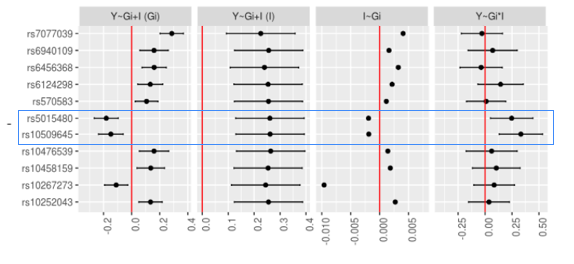
\includegraphics[width=.8\linewidth]{glu2}
    \label{fig:glu2}
    \begin{itemize}
      \item \textit{rs10509645} and \textit{rs5015480} locate in the intronic region of \textit{IDE} and \textit{HHEX} respectively (the genes are both T2D candidate genes)
      \item Their protective effect is masked by high fast glucose level
    \end{itemize}
  \end{frame}

%------------------------------------------------
\section{Discussion}
%------------------------------------------------

  \subsection{Summary}
  \begin{frame}
  \frametitle{Summary}
    \begin{itemize}
      \item We test the modifier effect of several intermediate trait on a subset of SNPs (GWAS hits or consistent SNPs)
      \item Overall, there are some interaction signals which indicates that the selected intermediate does as a whole modify the effect of some risk genes
      \item In particular,
        \begin{itemize}
          \item For GWAS hits, the epistatic effect either masks or enhances the effect of the locus when the baseline pathway level is high
          \item For consistent loci, the epistatic effect tend to mask the effect
        \end{itemize}
    \end{itemize}
  \end{frame}

  \subsection{Issues and future directions}
  \begin{frame}
  \frametitle{Issues and future directions}
    \begin{columns}
      \begin{column}{.39\textwidth}
        \begin{enumerate}
          \item Sample size is small and the interaction signal is weak
          \item Validate the signal
          \item Hard to interpret the result: what biological insight we can get out of such interaction
        \end{enumerate}
      \end{column}
      \begin{column}{.59\textwidth}
        \begin{enumerate}
          \item Use larger data sets (UK Biobank?)
          \item Seek some well-established epistasis in complex trait? Simulation analysis?
          \item Perform gene-based analysis. \textit{I.e.} to test the modifier effect of intermediate trait on how gene expression affect disease risk
        \end{enumerate}
      \end{column}
    \end{columns}
  \end{frame}

%------------------------------------------------

\begin{frame}
\Huge{\centerline{The End}}
\end{frame}

% %------------------------------------------------
% \section{Supplement}
% %------------------------------------------------
%
%   \subsection{Details of TargetFinder}
% 	\begin{frame} \label{sec:targetfinder_sup}
% 	\frametitle{Details of TargetFinder}
% 	\end{frame}

%------------------------------------------------
\begin{frame}[allowframebreaks]
\frametitle{References}
\footnotesize
\bibliography{mybib}
\bibliographystyle{plain}
\end{frame}

%----------------------------------------------------------------------------------------

\end{document}
